\section{Множество оптимальных стратегий}

\textbf{Утверждение}

Любая пара $(p^{*}, q^{*}) \in [0, 1]^{2}$ является оптимальной, т.е.  
$\forall$ $(p^{*}, q^{*}) \in [0, 1]^{2} \quad \exists$ $\mu, \lambda$: верно (7).
\vspace{5mm}

\textbf{Доказательство}

Зафиксируем некоторую пару  $(p^{*}, q^{*}) \in [0, 1]^{2}$ и найдя соответсвующие $\hat{\mu}(p^{*}, q^{*})$
 и $\hat{\lambda}(p^{*}, q^{*})$ покажем, что она является оптимальной.

\circled{1} Покажем оптимальность $p^{*}$:

Возьмём $\hat{\lambda}:=1-q^{*} \quad \Rightarrow$  поскольку 
$\argmin\limits_{p}L(p,q^{*},\hat{\lambda})=\forall$ при $ q^{*}=1-\hat{\lambda}$,

то и $p^{*} \in \argmin\limits_{p} L(p,q^{*},\hat{\lambda})$


\circled{2} Покажем оптимальность $q^{*}$:

\center
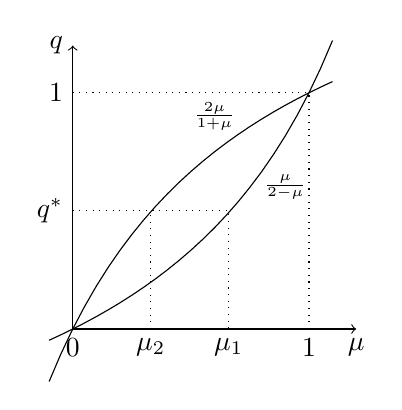
\begin{tikzpicture}[scale=3]

% horizontal axis
\draw[->] (0,0) -- (1.2,0) node[anchor=north] {$\mu$};
% labels
\draw	(0,0) node[anchor=north] {0}
		(1,0) node[anchor=north] {1}
		(0, 1) node[anchor=east] {1}
		(0, 0.5) node[anchor=east] {$q^{*}$}
		(0.33, 0) node[anchor=north] {$\mu_2$}
		(0.66, 0) node[anchor=north] {$\mu_1$};

% ranges
\draw	(0.9,0.6) node{{\scriptsize $\frac{\mu}{2-\mu}$}}
		(0.6,0.9) node{{\scriptsize $\frac{2\mu}{1+\mu}$}};

% vertical axis
\draw[->] (0,0) -- (0,1.2) node[anchor=east] {$q$};
% nominal speed
\draw[dotted] (1,0) -- (1,1) -- (0, 1);
\draw[dotted] (0,0.5) -- (0.66,0.5) -- (0.66, 0);
\draw[dotted] (0.33,0) -- (0.33,0.5);

% Psis
\draw[domain=-0.1:1.1] plot({\x}, {\x / (2 - \x)});
\draw[domain=-0.1:1.1] plot({\x}, {2 * \x / (1 + \x)});

\end{tikzpicture}
\begin{flushleft}

По имеющемуся $q^{*}$ решим уравнения $f_1(\mu_1)=q^{*}$ и $f_2(\mu_2)=q^{*}$, где
$f_1=\frac{\mu}{2-\mu}$ и $f_2=\frac{2\mu}{1+\mu}$:

$$q^{*}=\frac{2\mu_2}{1+\mu_2} \Rightarrow \mu_2=\frac{q^{*}}{2-q^{*}}$$

$$q^{*}=\frac{\mu_1}{2-\mu_1} \Rightarrow \mu_1=\frac{2q^{*}}{1+q^{*}}$$
Заметим, что при $q^{*} \in [0, 1] \quad \mu_2 \leq \mu_1$ 

В таком случае поскольку $1-p^{*} \in [0, 1]$, то при фиксированных переменных 
$(p^{*}, q^{*})$ будет реализован один и только один из 3-х вариантов:

1) $1-p^{*} \leq \mu_2$
  
2) $\mu_2 < 1-p^{*} \leq \mu_1$

3) $\mu_1 < 1-p^{*}$
\vspace{5mm}

1) $1-p^{*} \leq \mu_2$, т.е.  $1-p^{*} \leq \frac{q^{*}}{2-q^{*}}$, в таком случае
$\hat{\mu}:=\mu_1=\frac{2q^{*}}{1+q^{*}}$.

Действительно, при таком выборе $\hat{\mu}$ имеем:  $1-p^{*} \leq \mu_2 \leq \mu_1 = \hat{\mu} \Rightarrow$
$p^{*}+\hat{\mu}-1 \geq 0 \Rightarrow \argmax\limits_{q}M(p^{*},q,\hat{\mu})=
\frac{\hat{\mu}}{2-\hat{\mu}}=\frac{\mu_1}{2-\mu_1}$=
$\frac{\frac{2q^{*}}{1+q^{*}}}{2-\frac{2q^{*}}{1+q^{*}}}=q^{*} \Rightarrow$ 
\[
\textrm{при}
\begin{cases}
\hat{\mu}=\frac{2q^{*}}{1+q^{*}} \\
\hat{\lambda} = 1 - q^{*} \\
1-p^{*} \leq \frac{q^{*}}{2-q^{*}}
\end{cases}
(p^{*}, q^{*}) - \textrm{оптимальная пара}
\] 

2) $\mu_2 < 1-p^{*} \leq \mu_1$, т.е.  $\frac{q^{*}}{2-q^{*}} < 1-p^{*} \leq \frac{2q^{*}}{1+q^{*}}$,
в таком случае $\hat{\mu}:=\mu_1=\frac{2q^{*}}{1+q^{*}}$.
Действительно, при таком выборе $\hat{\mu}$ имеем :$1-p^{*} \leq \mu_1 = \hat{\mu} \Rightarrow$
$p^{*}+\hat{\mu}-1 \geq 0 \Rightarrow \argmax\limits_{q}M(p^{*},q,\hat{\mu})=
\frac{\hat{\mu}}{2-\hat{\mu}}=\frac{\mu_1}{2-\mu_1}$=
$\frac{\frac{2q^{*}}{1+q^{*}}}{2-\frac{2q^{*}}{1+q^{*}}}=q^{*} \Rightarrow$ 
\[
\textrm{при}
\begin{cases}
\hat{\mu}=\frac{2q^{*}}{1+q^{*}} \\
\hat{\lambda} = 1 - q^{*} \\
\frac{q^{*}}{2-1^{*}} < 1-p^{*} \leq \frac{2q^{*}}{1+q^{*}}
\end{cases}
(p^{*}, q^{*}) - \textrm{оптимальная пара}
\] 

3) $\mu_1 \leq 1-p^{*}$ т.е. $\frac{2q^{*}}{1+q^{*}} < 1-p^{*}$
в таком случае $\hat{\mu}=\mu_2=\frac{q^{*}}{2-q^{*}}$ 

действительно, при таком выборе $\hat{\mu}$ имеем $1-p^{*} \geq \mu_2 = \hat\mu \Rightarrow$
$p^{*}+\mu-1 \leq 0 \Rightarrow \argmax\limits_{q}M(p^{*},q,\hat{\mu})=
\frac{2\hat\mu}{1+\hat\mu}=\frac{2\mu_2}{1+\mu_2}=\frac{2\frac{q^{*}}{2-q^{*}}}{1+\frac{q^{*}}{2-q^{*}}}=
q^{*} \Rightarrow$ 
\[
\textrm{при}
\begin{cases}
\hat\mu=\frac{q^{*}}{2-q^{*}} \\
\hat\lambda = 1 - q^{*} \\
\frac{2q^{*}}{1+q^{*}} < 1-p^{*}
\end{cases}
(p^{*}, q^{*}) - \textrm{оптимальная пара}
\] 

Таким образом при имеющихся $(p^{*},q^{*})$ сначала надо определить в какой из вариантов 1-3 пара попадает, затем
по соответсвующим равенствам найти $\hat\mu$ и $\hat\lambda$.

\textbf{Утверждение доказано.}
\end{flushleft}
